\documentclass{article}\usepackage[]{graphicx}\usepackage[]{color}
%% maxwidth is the original width if it is less than linewidth
%% otherwise use linewidth (to make sure the graphics do not exceed the margin)
\makeatletter
\def\maxwidth{ %
  \ifdim\Gin@nat@width>\linewidth
    \linewidth
  \else
    \Gin@nat@width
  \fi
}
\makeatother

\definecolor{fgcolor}{rgb}{0.345, 0.345, 0.345}
\newcommand{\hlnum}[1]{\textcolor[rgb]{0.686,0.059,0.569}{#1}}%
\newcommand{\hlstr}[1]{\textcolor[rgb]{0.192,0.494,0.8}{#1}}%
\newcommand{\hlcom}[1]{\textcolor[rgb]{0.678,0.584,0.686}{\textit{#1}}}%
\newcommand{\hlopt}[1]{\textcolor[rgb]{0,0,0}{#1}}%
\newcommand{\hlstd}[1]{\textcolor[rgb]{0.345,0.345,0.345}{#1}}%
\newcommand{\hlkwa}[1]{\textcolor[rgb]{0.161,0.373,0.58}{\textbf{#1}}}%
\newcommand{\hlkwb}[1]{\textcolor[rgb]{0.69,0.353,0.396}{#1}}%
\newcommand{\hlkwc}[1]{\textcolor[rgb]{0.333,0.667,0.333}{#1}}%
\newcommand{\hlkwd}[1]{\textcolor[rgb]{0.737,0.353,0.396}{\textbf{#1}}}%

\usepackage{framed}
\makeatletter
\newenvironment{kframe}{%
 \def\at@end@of@kframe{}%
 \ifinner\ifhmode%
  \def\at@end@of@kframe{\end{minipage}}%
  \begin{minipage}{\columnwidth}%
 \fi\fi%
 \def\FrameCommand##1{\hskip\@totalleftmargin \hskip-\fboxsep
 \colorbox{shadecolor}{##1}\hskip-\fboxsep
     % There is no \\@totalrightmargin, so:
     \hskip-\linewidth \hskip-\@totalleftmargin \hskip\columnwidth}%
 \MakeFramed {\advance\hsize-\width
   \@totalleftmargin\z@ \linewidth\hsize
   \@setminipage}}%
 {\par\unskip\endMakeFramed%
 \at@end@of@kframe}
\makeatother

\definecolor{shadecolor}{rgb}{.97, .97, .97}
\definecolor{messagecolor}{rgb}{0, 0, 0}
\definecolor{warningcolor}{rgb}{1, 0, 1}
\definecolor{errorcolor}{rgb}{1, 0, 0}
\newenvironment{knitrout}{}{} % an empty environment to be redefined in TeX

\usepackage{alltt}
\usepackage{enumerate}
\usepackage{amsmath}
\IfFileExists{upquote.sty}{\usepackage{upquote}}{}
\begin{document}

\title{\huge \textbf{Stat 207 HW6} \\}
\author{\large Cheng Luo 912466499 \\ \large Fan Wu 912538518}
\maketitle

\newpage
\mbox{}
\newpage

\section{14.9}

\begin{enumerate}[(a)]

\item

\begin{knitrout}
\definecolor{shadecolor}{rgb}{0.969, 0.969, 0.969}\color{fgcolor}\begin{kframe}
\begin{alltt}
  \hlstd{dat} \hlkwb{=} \hlkwd{read.table}\hlstd{(}\hlstr{"CH14PR09.txt"}\hlstd{)}
  \hlkwd{names}\hlstd{(dat)} \hlkwb{=} \hlkwd{c}\hlstd{(}\hlstr{"Y"}\hlstd{,} \hlstr{"X"}\hlstd{)}
  \hlstd{logit} \hlkwb{=} \hlkwd{glm}\hlstd{(Y} \hlopt{~} \hlstd{X,} \hlkwc{data} \hlstd{= dat,} \hlkwc{family} \hlstd{=} \hlstr{"binomial"}\hlstd{)}
  \hlkwd{summary}\hlstd{(logit)}
\end{alltt}
\begin{verbatim}
## 
## Call:
## glm(formula = Y ~ X, family = "binomial", data = dat)
## 
## Deviance Residuals: 
##     Min       1Q   Median       3Q      Max  
## -1.7845  -0.8350   0.5065   0.8371   1.7145  
## 
## Coefficients:
##               Estimate Std. Error z value Pr(>|z|)  
## (Intercept) -10.308925   4.376997  -2.355   0.0185 *
## X             0.018920   0.007877   2.402   0.0163 *
## ---
## Signif. codes:  0 '***' 0.001 '**' 0.01 '*' 0.05 '.' 0.1 ' ' 1
## 
## (Dispersion parameter for binomial family taken to be 1)
## 
##     Null deviance: 37.393  on 26  degrees of freedom
## Residual deviance: 29.242  on 25  degrees of freedom
## AIC: 33.242
## 
## Number of Fisher Scoring iterations: 4
\end{verbatim}
\begin{alltt}
  \hlstd{b0} \hlkwb{=} \hlkwd{coef}\hlstd{(logit)[}\hlnum{1}\hlstd{]; b0}
\end{alltt}
\begin{verbatim}
## (Intercept) 
##   -10.30893
\end{verbatim}
\begin{alltt}
  \hlstd{b1} \hlkwb{=} \hlkwd{coef}\hlstd{(logit)[}\hlnum{2}\hlstd{]; b1}
\end{alltt}
\begin{verbatim}
##          X 
## 0.01891983
\end{verbatim}
\end{kframe}
\end{knitrout}

\qquad From the summary, the maximum likelihood estimates of $b_0 = -10.308925$, $b_1 = 0.018920$, $$\hat{\pi} = \frac{exp(b_0+b_1 X)}{1+exp(b_0+b_1 X)}=\frac{exp(-10.308925+0.018920 X)}{1+exp(-10.308925+0.018920 X)}$$

\item

\begin{knitrout}
\definecolor{shadecolor}{rgb}{0.969, 0.969, 0.969}\color{fgcolor}\begin{kframe}
\begin{alltt}
  \hlkwd{plot}\hlstd{(dat}\hlopt{$}\hlstd{X, dat}\hlopt{$}\hlstd{Y)}
  \hlkwd{points}\hlstd{(dat}\hlopt{$}\hlstd{X,} \hlkwd{fitted}\hlstd{(logit),} \hlkwc{type} \hlstd{=} \hlstr{'l'}\hlstd{,} \hlkwc{lty} \hlstd{=} \hlnum{1}\hlstd{)}
  \hlkwd{points}\hlstd{(dat}\hlopt{$}\hlstd{X,} \hlkwd{lowess}\hlstd{(dat}\hlopt{$}\hlstd{X, dat}\hlopt{$}\hlstd{Y)}\hlopt{$}\hlstd{y,} \hlkwc{type} \hlstd{=} \hlstr{'l'}\hlstd{,} \hlkwc{lty} \hlstd{=} \hlnum{2}\hlstd{)}
  \hlkwd{legend}\hlstd{(}\hlstr{'right'}\hlstd{,} \hlkwc{legend} \hlstd{=} \hlkwd{c}\hlstd{(}\hlstr{'fitted'}\hlstd{,} \hlstr{'lowess'}\hlstd{),}
       \hlkwc{lty} \hlstd{=} \hlnum{1}\hlopt{:}\hlnum{2}\hlstd{)}
\end{alltt}
\end{kframe}
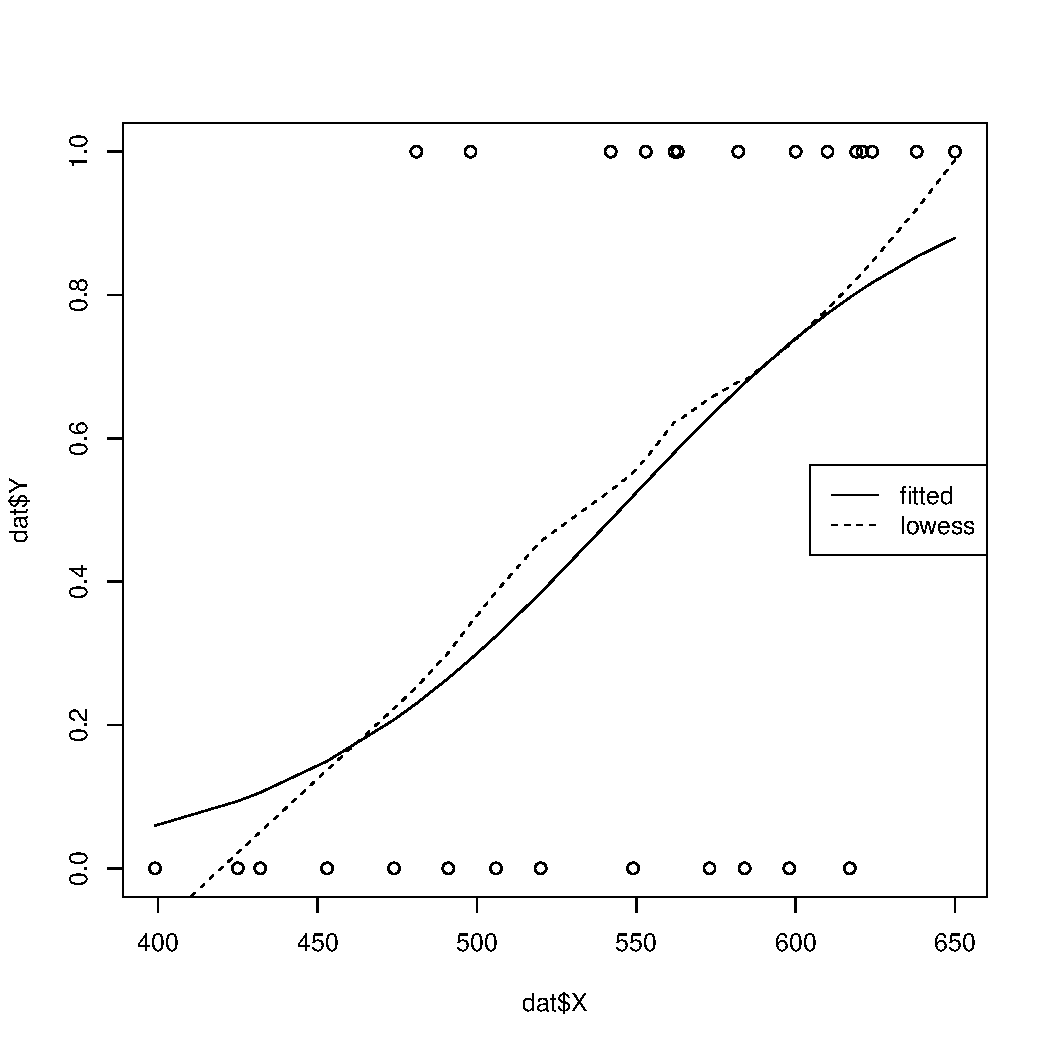
\includegraphics[width=\maxwidth]{figure/unnamed-chunk-2-1} 

\end{knitrout}

\qquad The fitted logistic response function appears to be well.

\item

\begin{knitrout}
\definecolor{shadecolor}{rgb}{0.969, 0.969, 0.969}\color{fgcolor}\begin{kframe}
\begin{alltt}
  \hlkwd{exp}\hlstd{(}\hlnum{0.018920}\hlstd{)}
\end{alltt}
\begin{verbatim}
## [1] 1.0191
\end{verbatim}
\end{kframe}
\end{knitrout}

\qquad $exp(\beta_1)=1.0191$, so that the odds of employee's ability increased by 1.91\% with each additional employee's emotional stability.

\item

\begin{knitrout}
\definecolor{shadecolor}{rgb}{0.969, 0.969, 0.969}\color{fgcolor}\begin{kframe}
\begin{alltt}
  \hlstd{newdat} \hlkwb{=} \hlkwd{data.frame}\hlstd{(}\hlkwc{X} \hlstd{=} \hlnum{550}\hlstd{)}
  \hlkwd{predict}\hlstd{(logit,} \hlkwc{newdata} \hlstd{= newdat,} \hlkwc{type} \hlstd{=} \hlstr{"response"}\hlstd{)}
\end{alltt}
\begin{verbatim}
##         1 
## 0.5242263
\end{verbatim}
\end{kframe}
\end{knitrout}

\qquad The estimated probability that employees with an emotional stability test score of 550 will be able to perform in a task group is 0.5242263 .

\end{enumerate}

\section{Problem 5}

\begin{enumerate}[(a)]

\item

\begin{knitrout}
\definecolor{shadecolor}{rgb}{0.969, 0.969, 0.969}\color{fgcolor}\begin{kframe}
\begin{alltt}
  \hlstd{dat} \hlkwb{=} \hlkwd{read.table}\hlstd{(}\hlstr{"apartment.txt"}\hlstd{,} \hlkwc{header} \hlstd{=} \hlnum{TRUE}\hlstd{)}
  \hlkwd{require}\hlstd{(}\hlstr{"pls"}\hlstd{)}
\end{alltt}


{\ttfamily\noindent\itshape\color{messagecolor}{\#\# Loading required package: pls}}

{\ttfamily\noindent\color{warningcolor}{\#\# Warning: package 'pls' was built under R version 3.1.2}}

{\ttfamily\noindent\itshape\color{messagecolor}{\#\# \\\#\# Attaching package: 'pls'\\\#\# \\\#\# The following object is masked from 'package:stats':\\\#\# \\\#\#\ \ \ \  loadings}}\begin{alltt}
  \hlstd{dat.stan} \hlkwb{=} \hlstd{dat}
  \hlkwa{for}\hlstd{(j} \hlkwa{in} \hlnum{1}\hlopt{:}\hlkwd{ncol}\hlstd{(dat))}
    \hlstd{dat.stan[,j]} \hlkwb{=} \hlstd{(dat[,j]} \hlopt{-} \hlkwd{mean}\hlstd{(dat[,j]))}\hlopt{/}\hlkwd{sd}\hlstd{(dat[,j])}
  \hlstd{n} \hlkwb{=} \hlkwd{nrow}\hlstd{(dat); n}
\end{alltt}
\begin{verbatim}
## [1] 25
\end{verbatim}
\begin{alltt}
  \hlstd{fit} \hlkwb{=} \hlkwd{plsr}\hlstd{(Y} \hlopt{~}\hlnum{0} \hlopt{+} \hlstd{.,} \hlkwc{data} \hlstd{= dat.stan,} \hlnum{5}\hlstd{,} \hlkwc{validation} \hlstd{=} \hlstr{"CV"}\hlstd{)}
  \hlkwd{summary}\hlstd{(fit)}
\end{alltt}
\begin{verbatim}
## Data: 	X dimension: 25 5 
## 	Y dimension: 25 1
## Fit method: kernelpls
## Number of components considered: 5
## 
## VALIDATION: RMSEP
## Cross-validated using 10 random segments.
##        (Intercept)  1 comps  2 comps  3 comps  4 comps  5 comps
## CV           1.021   0.4301   0.2754   0.2000   0.1800   0.1814
## adjCV        1.021   0.4113   0.2699   0.1946   0.1768   0.1785
## 
## TRAINING: % variance explained
##    1 comps  2 comps  3 comps  4 comps  5 comps
## X    52.58    66.94    85.17    91.35   100.00
## Y    92.14    96.53    97.92    98.01    98.05
\end{verbatim}
\begin{alltt}
  \hlkwd{scores}\hlstd{(fit)}
\end{alltt}
\begin{verbatim}
##         Comp 1      Comp 2      Comp 3       Comp 4       Comp 5
## 1  -1.43809414  0.31257891 -0.66465691 -0.238439173  0.159569798
## 2   1.65010464 -1.22067017 -0.64427193  0.663274381 -0.865798881
## 3  -1.05278777  0.23602481 -0.31050170 -0.020291335  0.008296669
## 4   2.04913072  1.58847399  1.43430866  0.056609088  0.998283179
## 5  -1.13936477  0.29816779  0.09920242 -0.077974453 -0.315614625
## 6   0.43417694 -0.26004572 -1.00952515  0.650608213  0.643434804
## 7  -1.22623584 -0.17772037 -1.20001375 -0.068573074  0.280347608
## 8  -0.65767426  0.36330099  1.03967609 -0.268877399 -1.370326788
## 9   1.42140486 -1.39664727  1.71050459 -0.349167349  1.208806076
## 10  5.48855488  0.07922404 -1.42064358 -0.711330743 -0.865767632
## 11  1.98211289  1.07654279 -0.19360273  0.247458345  0.426744426
## 12  0.04614307 -0.64535432  0.61846253 -0.480354282  1.057377814
## 13 -0.71466027  0.75759510 -0.14154088 -0.168335371  0.116132220
## 14 -0.89066011 -0.24878365  1.32675710 -0.194652611 -0.421211010
## 15  0.41103483 -1.04629327  0.48064460  0.246649352  0.306896982
## 16 -1.02148397 -0.21942028  1.30789234 -0.154167563 -0.564857509
## 17  0.77416093 -0.20479803 -0.70800362 -0.161374329 -0.174850186
## 18 -1.24116621  0.12113528 -0.52207912 -0.071041829  0.036778165
## 19 -0.36723658 -0.32047183  0.43733622  0.267294081 -0.910453651
## 20 -1.18318143  0.27366081  0.02535909 -0.014259103 -0.184750720
## 21 -1.21222218 -0.07162508 -1.09128123 -0.058437672  0.309847588
## 22 -1.43423671  0.17603426  0.16663071 -0.203393131 -0.594314019
## 23  1.20087805  0.46813038  1.30158137  0.899514178 -0.313846232
## 24 -1.14387561 -0.16195504 -1.19339577 -0.004177028  0.359346058
## 25 -0.73482194  0.22291589 -0.84883933  0.213438810  0.669929866
## attr(,"class")
## [1] "scores"
## attr(,"explvar")
##    Comp 1    Comp 2    Comp 3    Comp 4    Comp 5 
## 52.582242 14.361573 18.228133  6.180191  8.647861
\end{verbatim}
\begin{alltt}
  \hlkwd{loadings}\hlstd{(fit)[,} \hlnum{1}\hlopt{:}\hlnum{3}\hlstd{]}
\end{alltt}
\begin{verbatim}
##         Comp 1     Comp 2      Comp 3
## X1 -0.07983743  0.6903977 -0.76418606
## X2  0.59805736  0.1008482 -0.08164449
## X3  0.54164949 -0.5440785 -0.25282151
## X4  0.16890957 -0.7416964  0.59414237
## X5  0.56738864  0.5744813  0.04300711
\end{verbatim}
\begin{alltt}
  \hlstd{k} \hlkwb{=} \hlnum{1}\hlopt{:}\hlnum{6}
  \hlstd{r.sq} \hlkwb{=} \hlkwd{c}\hlstd{(}\hlnum{92.14} \hlstd{,}   \hlnum{96.53}  \hlstd{,}  \hlnum{97.92}  \hlstd{,}  \hlnum{98.01} \hlstd{,}   \hlnum{98.05}\hlstd{)}\hlopt{/}\hlnum{100}
  \hlstd{r.adj} \hlkwb{=} \hlnum{1} \hlopt{-} \hlstd{(n}\hlopt{-}\hlnum{1}\hlstd{)}\hlopt{/}\hlstd{(n}\hlopt{-}\hlstd{k}\hlopt{-}\hlnum{1}\hlstd{)}\hlopt{*}\hlstd{(}\hlnum{1}\hlopt{-}\hlstd{r.sq); r.adj}
\end{alltt}


{\ttfamily\noindent\color{warningcolor}{\#\# Warning in (n - 1)/(n - k - 1) * (1 - r.sq): longer object length is not a multiple of shorter object length}}\begin{verbatim}
## [1] 0.9179826 0.9621455 0.9762286 0.9761200 0.9753684 0.8952000
\end{verbatim}
\begin{alltt}
  \hlkwd{plot}\hlstd{(fit,} \hlkwc{plottype} \hlstd{=} \hlstr{"scores"}\hlstd{,} \hlkwc{comps} \hlstd{=} \hlnum{1}\hlopt{:}\hlnum{3}\hlstd{)}
\end{alltt}
\end{kframe}
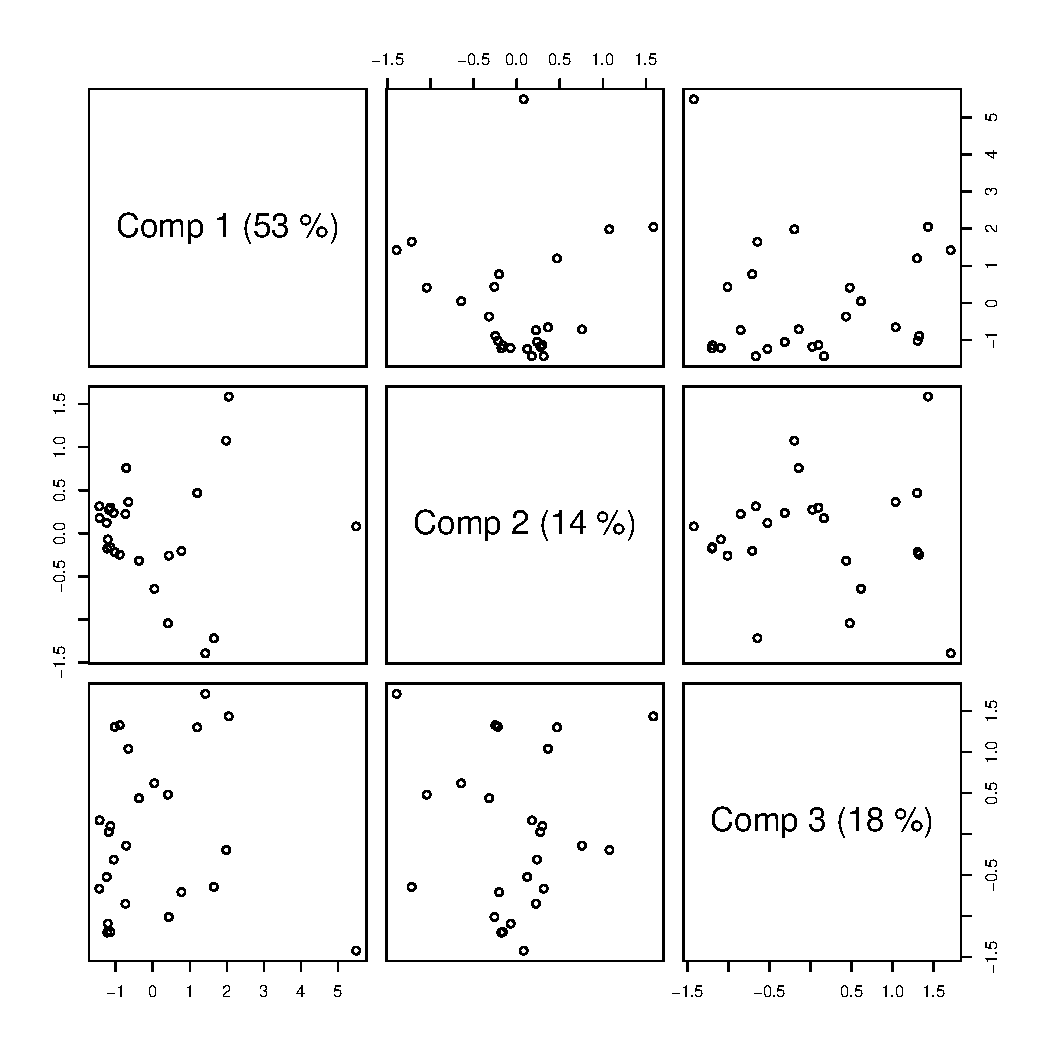
\includegraphics[width=\maxwidth]{figure/unnamed-chunk-5-1} 

\end{knitrout}

\item

\begin{knitrout}
\definecolor{shadecolor}{rgb}{0.969, 0.969, 0.969}\color{fgcolor}\begin{kframe}
\begin{alltt}
  \hlstd{r.sq} \hlkwb{=} \hlkwd{c}\hlstd{(}\hlnum{0}\hlstd{, r.sq); r.sq}
\end{alltt}
\begin{verbatim}
## [1] 0.0000 0.9214 0.9653 0.9792 0.9801 0.9805
\end{verbatim}
\begin{alltt}
  \hlstd{f.k} \hlkwb{=} \hlkwd{sapply}\hlstd{(}\hlnum{2}\hlopt{:}\hlkwd{length}\hlstd{(r.sq),} \hlkwa{function}\hlstd{(}\hlkwc{k}\hlstd{)}
    \hlstd{(n}\hlopt{-}\hlstd{k}\hlopt{-}\hlnum{1}\hlstd{)}\hlopt{*}\hlstd{(r.sq[k]} \hlopt{-} \hlstd{r.sq[k}\hlopt{-}\hlnum{1}\hlstd{])}\hlopt{/}\hlstd{(}\hlnum{1}\hlopt{-}\hlstd{r.sq[k])); f.k}
\end{alltt}
\begin{verbatim}
## [1] 257.8982188  26.5677233  13.3653846   0.8592965   0.3692308
\end{verbatim}
\begin{alltt}
  \hlkwd{qf}\hlstd{(}\hlnum{1}\hlopt{-}\hlnum{0.05}\hlstd{,} \hlnum{1}\hlstd{,} \hlnum{1}\hlopt{:}\hlnum{5}\hlstd{)}
\end{alltt}
\begin{verbatim}
## [1] 161.447639  18.512821  10.127964   7.708647   6.607891
\end{verbatim}
\end{kframe}
\end{knitrout}

\qquad As we can see from above, we might decide the number of components to keep is 3.

\item

\begin{knitrout}
\definecolor{shadecolor}{rgb}{0.969, 0.969, 0.969}\color{fgcolor}\begin{kframe}
\begin{alltt}
  \hlstd{model} \hlkwb{=} \hlkwd{plsr}\hlstd{(Y} \hlopt{~} \hlnum{0} \hlopt{+} \hlstd{.,}
               \hlnum{3}\hlstd{,} \hlkwc{data} \hlstd{= dat.stan,} \hlkwc{validation} \hlstd{=} \hlstr{'CV'}\hlstd{)}
  \hlkwd{coef}\hlstd{(model)}
\end{alltt}
\begin{verbatim}
## , , 3 comps
## 
##              Y
## X1 -0.11356364
## X2  0.34543343
## X3 -0.02384503
## X4  0.05143543
## X5  0.67482746
\end{verbatim}
\begin{alltt}
  \hlkwd{plot}\hlstd{(}\hlkwd{fitted}\hlstd{(model)[,,}\hlnum{3}\hlstd{], dat.stan[,}\hlnum{1}\hlstd{])}
\end{alltt}
\end{kframe}
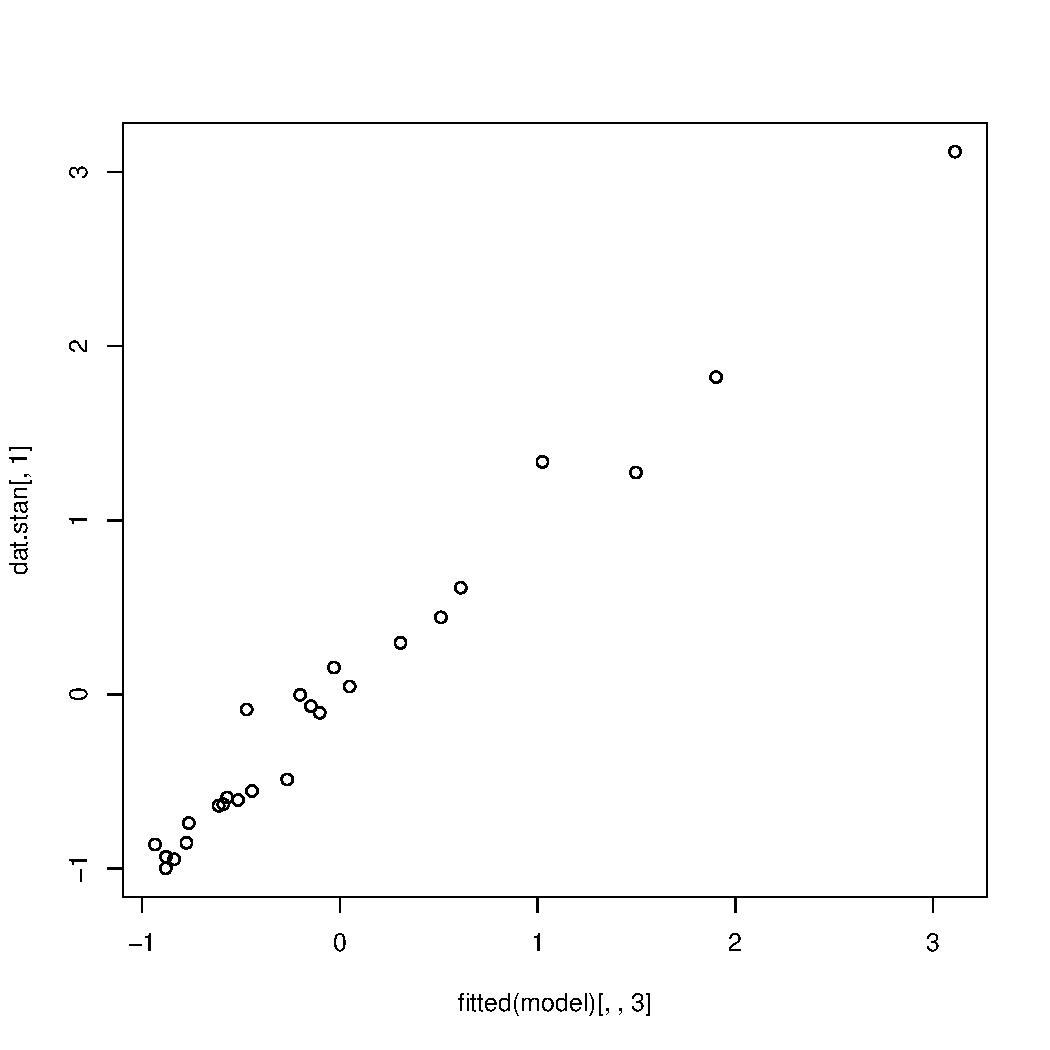
\includegraphics[width=\maxwidth]{figure/unnamed-chunk-7-1} 
\begin{kframe}\begin{alltt}
  \hlkwd{plot}\hlstd{(}\hlkwd{fitted}\hlstd{(model)[,,}\hlnum{3}\hlstd{],} \hlkwd{resid}\hlstd{(model)[,,}\hlnum{3}\hlstd{])}
\end{alltt}
\end{kframe}
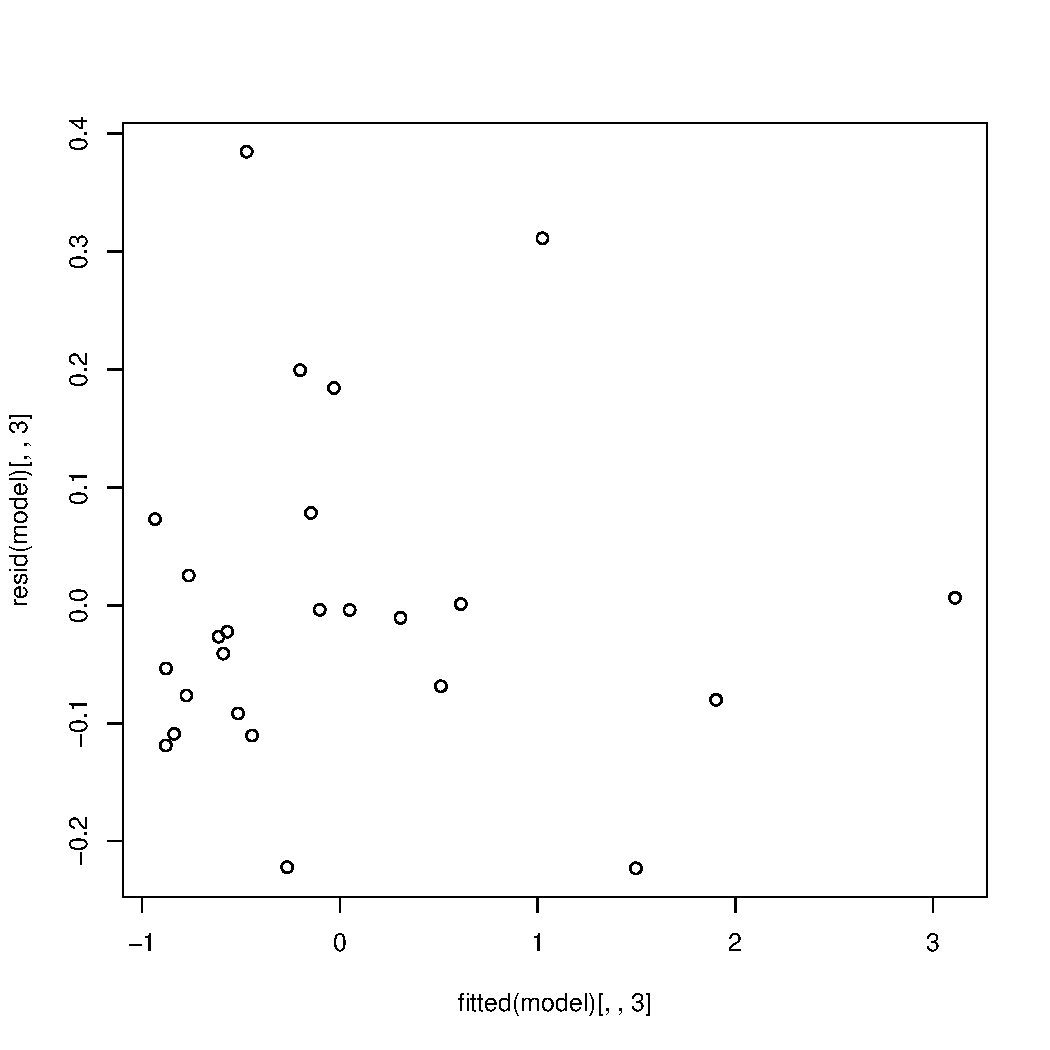
\includegraphics[width=\maxwidth]{figure/unnamed-chunk-7-2} 
\begin{kframe}\begin{alltt}
  \hlkwd{hist}\hlstd{(}\hlkwd{resid}\hlstd{(model)[,,}\hlnum{3}\hlstd{])}
\end{alltt}
\end{kframe}
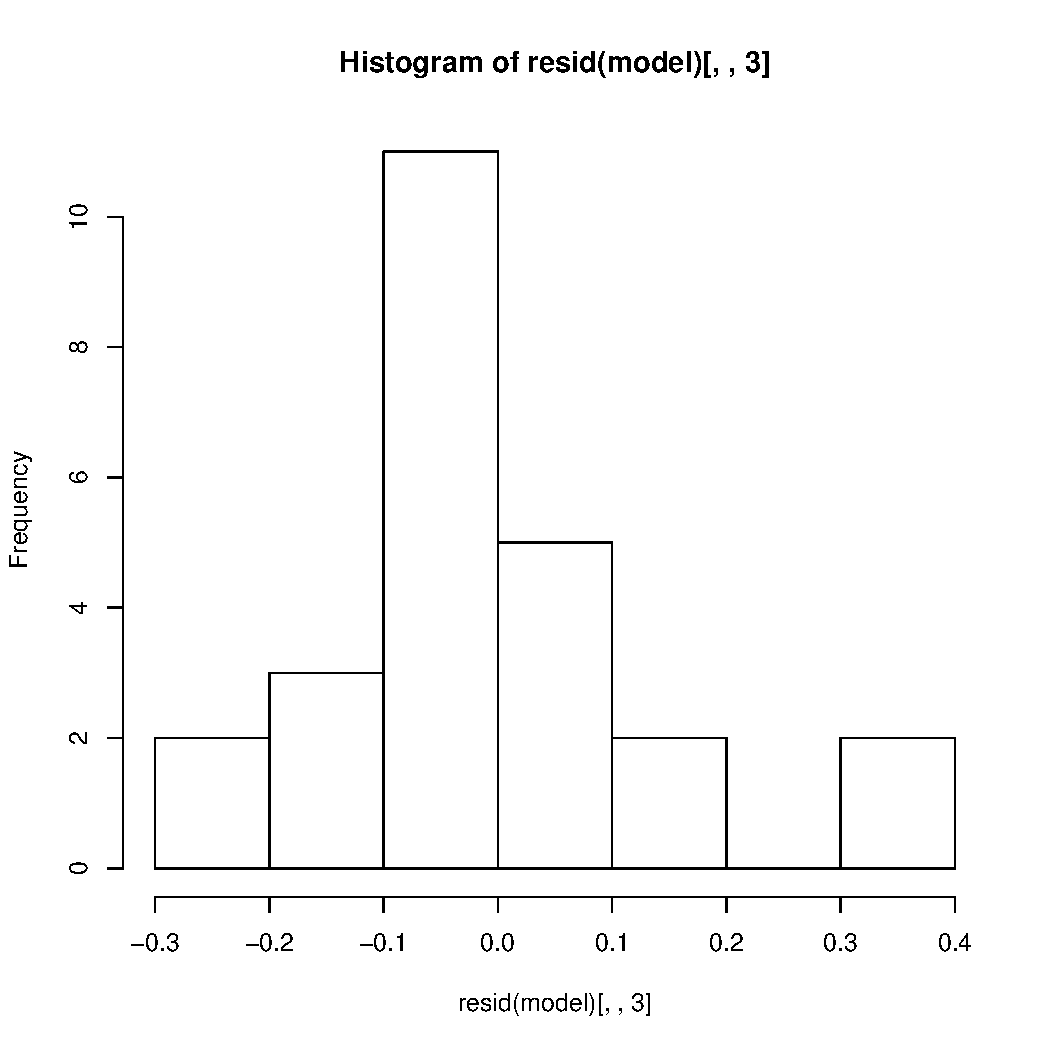
\includegraphics[width=\maxwidth]{figure/unnamed-chunk-7-3} 

\end{knitrout}

\qquad The final model is $$Y^* = -0.11356364 X_1^* + 0.34543343 X_2^* -0.02384503 X_3^* + 0.05143543 X_4^* +0.67482746 X_5^* $$
\qquad The observed against the fitted values plots shows it fits well, and residuals against the fitted values and the histogram of the residuals plots show it has no sign for unequal variance.

\end{enumerate}

\section{Problem 6}

\begin{enumerate}[(a)]

\item

\begin{knitrout}
\definecolor{shadecolor}{rgb}{0.969, 0.969, 0.969}\color{fgcolor}\begin{kframe}
\begin{alltt}
  \hlkwd{require}\hlstd{(glmnet)}
\end{alltt}


{\ttfamily\noindent\itshape\color{messagecolor}{\#\# Loading required package: glmnet}}

{\ttfamily\noindent\color{warningcolor}{\#\# Warning: package 'glmnet' was built under R version 3.1.2}}

{\ttfamily\noindent\itshape\color{messagecolor}{\#\# Loading required package: Matrix}}

{\ttfamily\noindent\color{warningcolor}{\#\# Warning: package 'Matrix' was built under R version 3.1.2}}

{\ttfamily\noindent\itshape\color{messagecolor}{\#\# Loaded glmnet 1.9-8}}\begin{alltt}
  \hlstd{x} \hlkwb{=} \hlkwd{as.matrix}\hlstd{(dat.stan[,} \hlopt{-}\hlnum{1}\hlstd{])}
  \hlstd{model} \hlkwb{=} \hlkwd{cv.glmnet}\hlstd{(x, dat.stan[,} \hlnum{1}\hlstd{],} \hlkwc{intercept} \hlstd{=} \hlnum{FALSE}\hlstd{)}
\end{alltt}


{\ttfamily\noindent\color{warningcolor}{\#\# Warning: Option grouped=FALSE enforced in cv.glmnet, since < 3 observations per fold}}\begin{alltt}
  \hlkwd{plot}\hlstd{(model)}
\end{alltt}
\end{kframe}
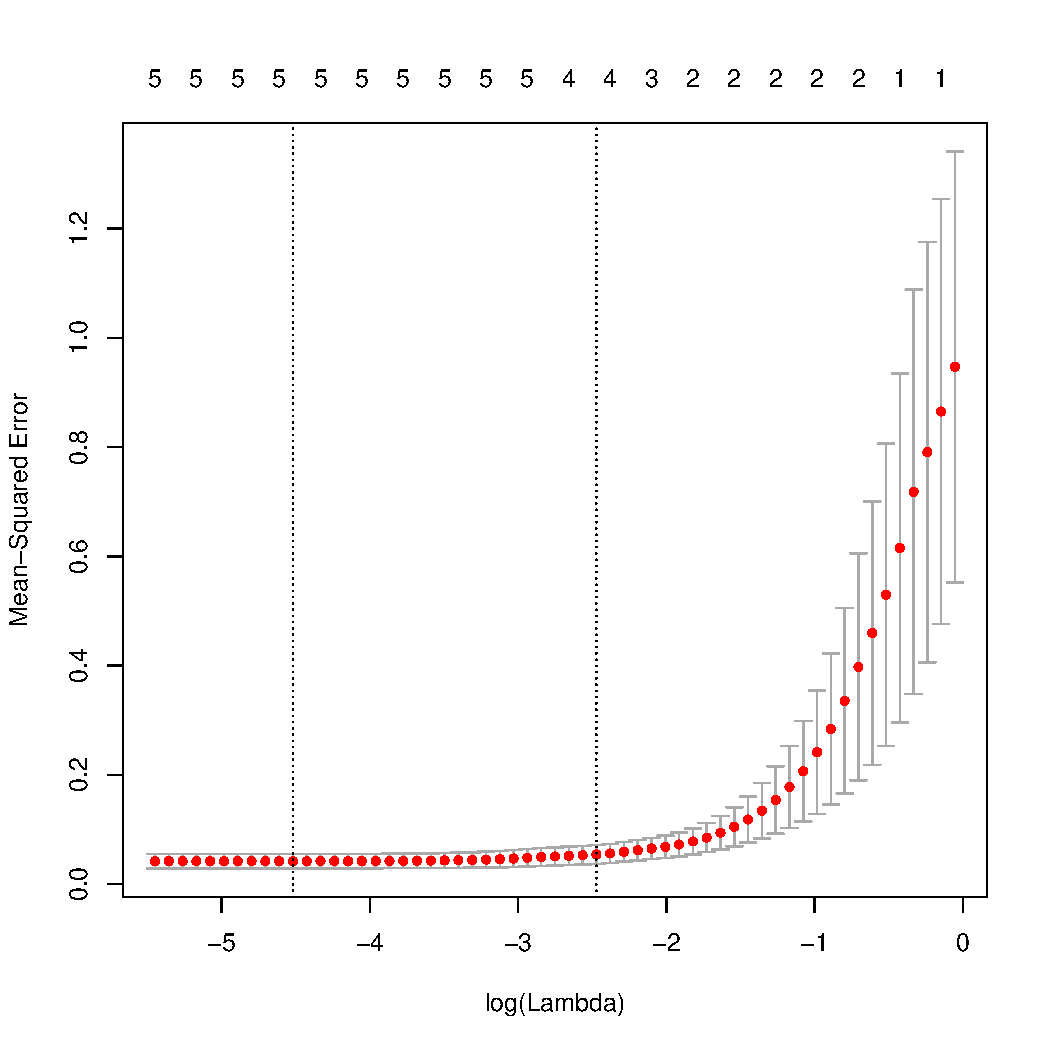
\includegraphics[width=\maxwidth]{figure/unnamed-chunk-8-1} 
\begin{kframe}\begin{alltt}
  \hlstd{model}\hlopt{$}\hlstd{lambda.min}
\end{alltt}
\begin{verbatim}
## [1] 0.01090626
\end{verbatim}
\end{kframe}
\end{knitrout}

\item

\begin{knitrout}
\definecolor{shadecolor}{rgb}{0.969, 0.969, 0.969}\color{fgcolor}\begin{kframe}
\begin{alltt}
  \hlkwd{coef}\hlstd{(model)}
\end{alltt}
\begin{verbatim}
## 6 x 1 sparse Matrix of class "dgCMatrix"
##                      1
## (Intercept)  .        
## X1          -0.0396032
## X2           0.2645694
## X3           .        
## X4           0.0070940
## X5           0.6501270
\end{verbatim}
\begin{alltt}
  \hlstd{fitted.} \hlkwb{=} \hlkwd{predict}\hlstd{(model,} \hlkwc{newx} \hlstd{= x)}
  \hlkwd{plot}\hlstd{(fitted., dat.stan[,}\hlnum{1}\hlstd{])}
\end{alltt}
\end{kframe}
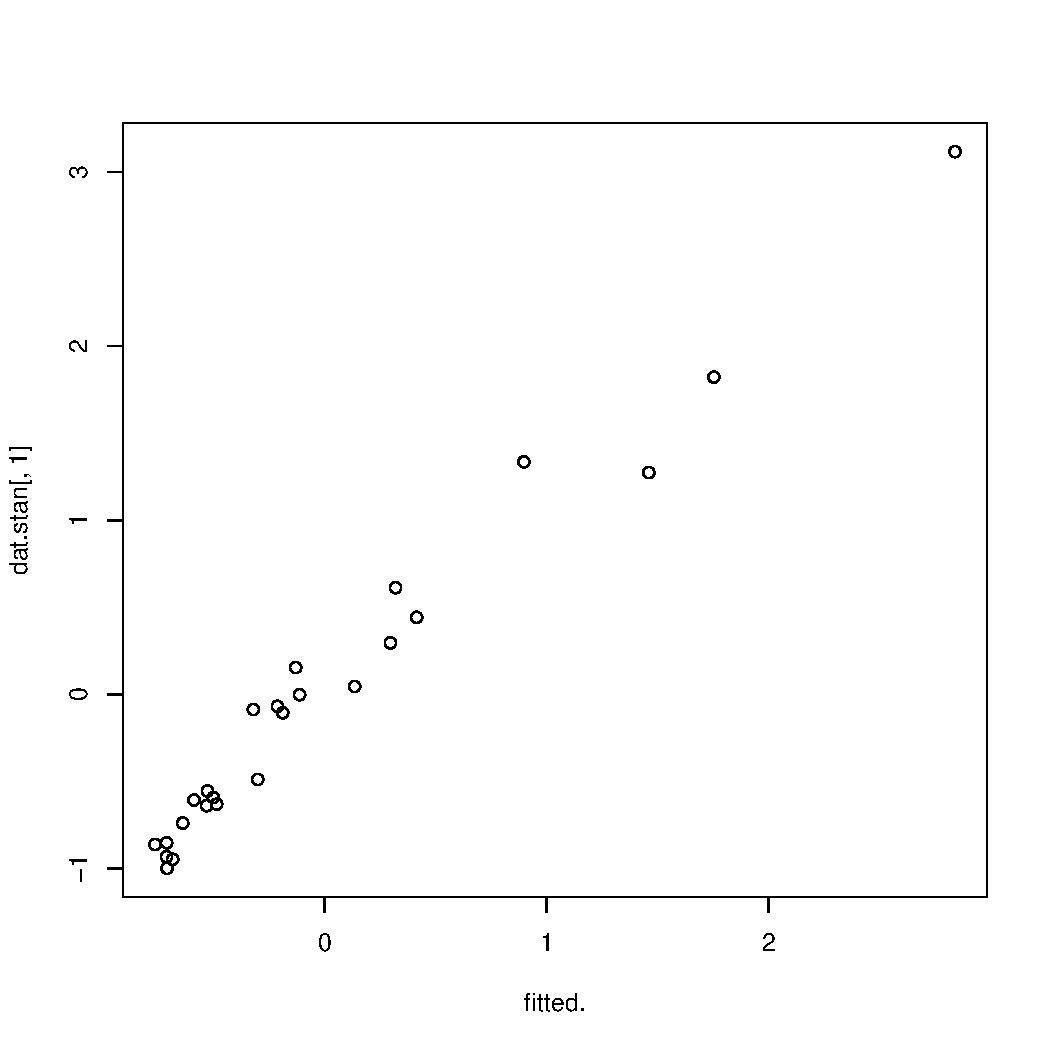
\includegraphics[width=\maxwidth]{figure/unnamed-chunk-9-1} 
\begin{kframe}\begin{alltt}
  \hlstd{res} \hlkwb{=} \hlstd{dat.stan[,}\hlnum{1}\hlstd{]} \hlopt{-} \hlstd{fitted.}
  \hlkwd{plot}\hlstd{(fitted., res)}
\end{alltt}
\end{kframe}
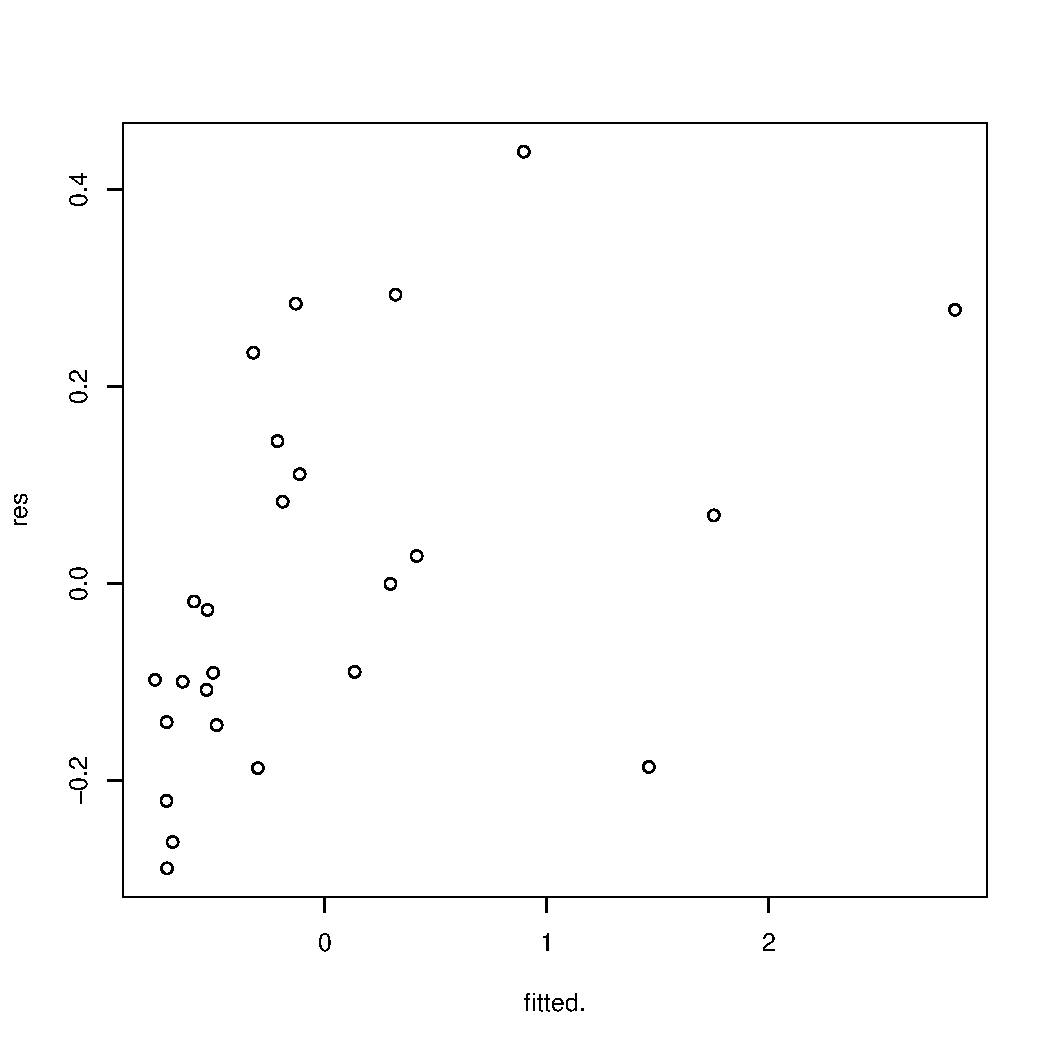
\includegraphics[width=\maxwidth]{figure/unnamed-chunk-9-2} 
\begin{kframe}\begin{alltt}
  \hlkwd{hist}\hlstd{(res)}
\end{alltt}
\end{kframe}
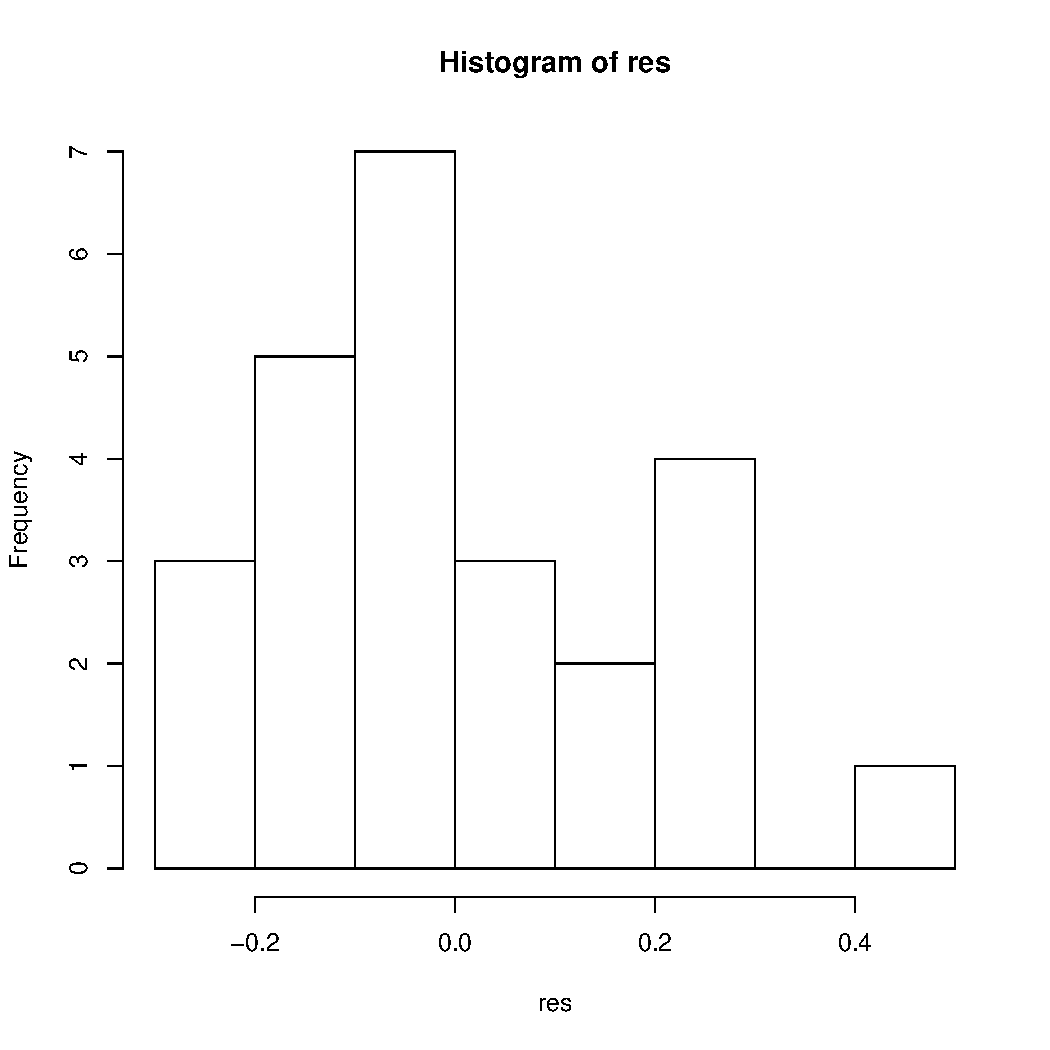
\includegraphics[width=\maxwidth]{figure/unnamed-chunk-9-3} 

\end{knitrout}

\qquad The final model is $$Y^* =  -0.0610260558 X_1^* + 0.2646220373 X_2^* + 0.0002055733 X_3^* + 0.0237525845 X_4^* +0.6758144083 X_5^* $$
\qquad The observed against the fitted values plots shows it fits well, and residuals against the fitted values and the histogram of the residuals plots show it has no sign for unequal variance.

\end{enumerate}

\section{Problem 7}

\section{Problem 8}

\begin{enumerate}[(a)]

\item

\begin{knitrout}
\definecolor{shadecolor}{rgb}{0.969, 0.969, 0.969}\color{fgcolor}\begin{kframe}
\begin{alltt}
  \hlstd{lambda} \hlkwb{=} \hlkwd{c}\hlstd{(}\hlnum{19}\hlstd{,} \hlnum{3}\hlstd{,} \hlnum{1}\hlstd{,} \hlnum{.7}\hlstd{,} \hlnum{.3}\hlstd{)}
  \hlstd{e.beta} \hlkwb{=} \hlkwd{c}\hlstd{(}\hlnum{.8}\hlstd{,} \hlnum{.3}\hlstd{,} \hlnum{.2}\hlstd{,} \hlnum{.2}\hlstd{,} \hlnum{.1}\hlstd{)}
  \hlstd{sig.sq} \hlkwb{=} \hlnum{2.5}

  \hlstd{k.seq} \hlkwb{=} \hlkwd{seq}\hlstd{(}\hlnum{0}\hlstd{,} \hlnum{1000}\hlstd{,} \hlnum{1}\hlstd{)}

  \hlstd{d.foo} \hlkwb{=} \hlkwa{function}\hlstd{(}\hlkwc{k}\hlstd{,} \hlkwc{sig.sq}\hlstd{,} \hlkwc{lambda}\hlstd{,} \hlkwc{e.beta}\hlstd{)}
  \hlstd{\{}
    \hlstd{sig.sq} \hlopt{*} \hlkwd{sum}\hlstd{( lambda} \hlopt{/} \hlstd{(k}\hlopt{+}\hlstd{lambda)}\hlopt{^}\hlnum{2} \hlstd{)} \hlopt{+}
      \hlstd{k}\hlopt{^}\hlnum{2} \hlopt{*} \hlkwd{sum}\hlstd{( e.beta}\hlopt{^}\hlnum{2} \hlopt{/} \hlstd{(k}\hlopt{+}\hlstd{lambda)}\hlopt{^}\hlnum{2} \hlstd{)}
  \hlstd{\}}

  \hlstd{d.eval} \hlkwb{=} \hlkwd{sapply}\hlstd{(k.seq,} \hlkwa{function}\hlstd{(}\hlkwc{k}\hlstd{)}
    \hlkwd{d.foo}\hlstd{(k, sig.sq, lambda, e.beta))}
  \hlkwd{plot}\hlstd{(k.seq, d.eval)}
\end{alltt}
\end{kframe}
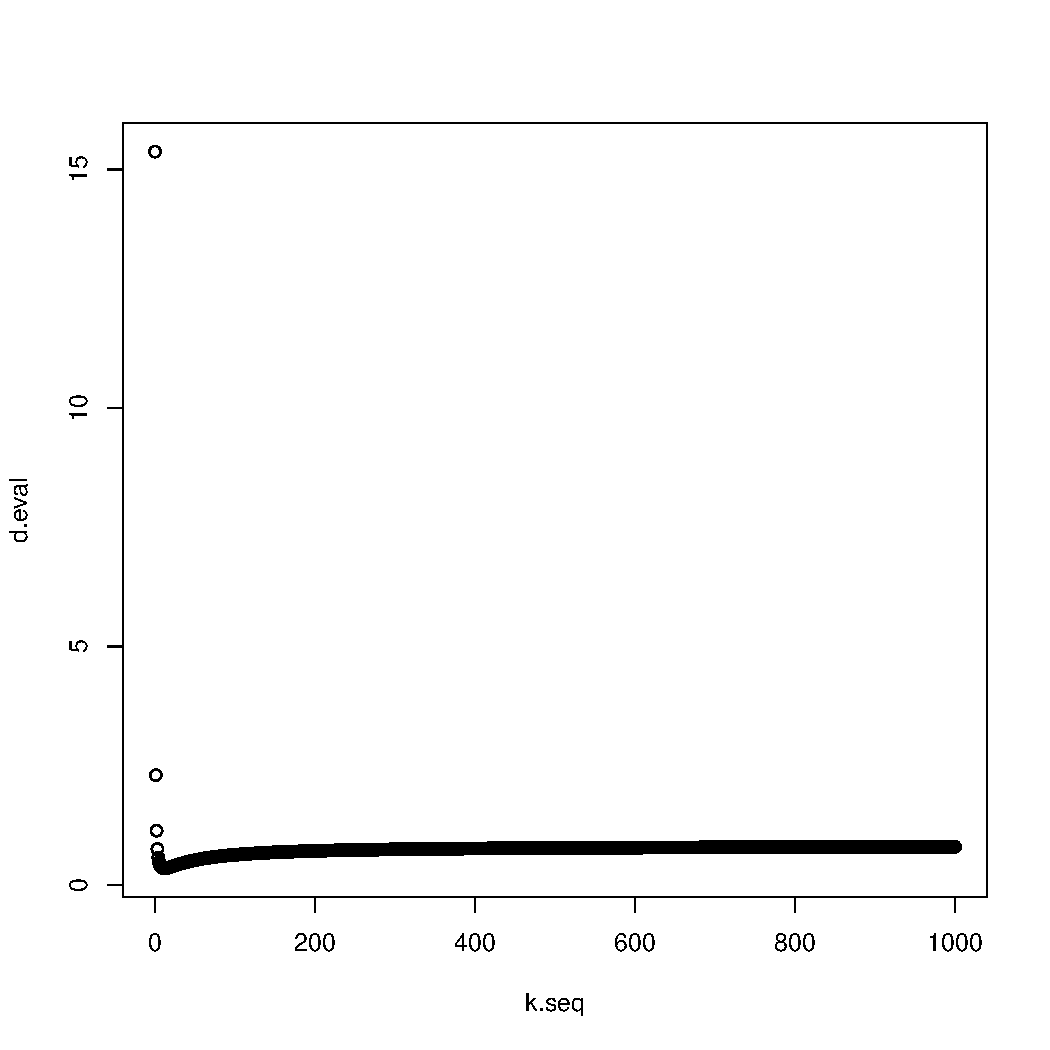
\includegraphics[width=\maxwidth]{figure/unnamed-chunk-10-1} 
\begin{kframe}\begin{alltt}
  \hlstd{d.opt} \hlkwb{=} \hlkwd{optimize}\hlstd{(d.foo,} \hlkwd{c}\hlstd{(}\hlnum{0}\hlstd{,} \hlnum{100}\hlstd{), sig.sq, lambda, e.beta); d.opt}
\end{alltt}
\begin{verbatim}
## $minimum
## [1] 11.94841
## 
## $objective
## [1] 0.346172
\end{verbatim}
\end{kframe}
\end{knitrout}

\item

\begin{knitrout}
\definecolor{shadecolor}{rgb}{0.969, 0.969, 0.969}\color{fgcolor}\begin{kframe}
\begin{alltt}
\hlstd{lambda} \hlkwb{=} \hlkwd{c}\hlstd{(}\hlnum{19}\hlstd{,} \hlnum{3}\hlstd{,} \hlnum{1}\hlstd{,} \hlnum{.7}\hlstd{,} \hlnum{.3}\hlstd{)}
\hlstd{e.beta} \hlkwb{=} \hlkwd{c}\hlstd{(}\hlnum{.8}\hlstd{,} \hlnum{.3}\hlstd{,} \hlnum{.2}\hlstd{,} \hlnum{.2}\hlstd{,} \hlnum{.1}\hlstd{)}
\hlstd{sig.sq} \hlkwb{=} \hlnum{2.5}

\hlstd{k.seq} \hlkwb{=} \hlkwd{seq}\hlstd{(}\hlnum{0}\hlstd{,} \hlnum{1000}\hlstd{,} \hlnum{1}\hlstd{)}

\hlstd{l.foo} \hlkwb{=} \hlkwa{function}\hlstd{(}\hlkwc{k}\hlstd{,} \hlkwc{sig.sq}\hlstd{,} \hlkwc{lambda}\hlstd{,} \hlkwc{e.beta}\hlstd{)}
\hlstd{\{}
  \hlstd{sig.sq} \hlopt{*} \hlkwd{sum}\hlstd{( lambda}\hlopt{^}\hlnum{2} \hlopt{/} \hlstd{(k}\hlopt{+}\hlstd{lambda)}\hlopt{^}\hlnum{2} \hlstd{)} \hlopt{+}
    \hlstd{k}\hlopt{^}\hlnum{2} \hlopt{*} \hlkwd{sum}\hlstd{( e.beta}\hlopt{^}\hlnum{2}\hlopt{*}\hlstd{lambda} \hlopt{/} \hlstd{(k}\hlopt{+}\hlstd{lambda)}\hlopt{^}\hlnum{2} \hlstd{)}
\hlstd{\}}

\hlstd{l.eval} \hlkwb{=} \hlkwd{sapply}\hlstd{(k.seq,} \hlkwa{function}\hlstd{(}\hlkwc{k}\hlstd{)}
  \hlkwd{l.foo}\hlstd{(k, sig.sq, lambda, e.beta))}
\hlkwd{plot}\hlstd{(k.seq, l.eval)}
\end{alltt}
\end{kframe}
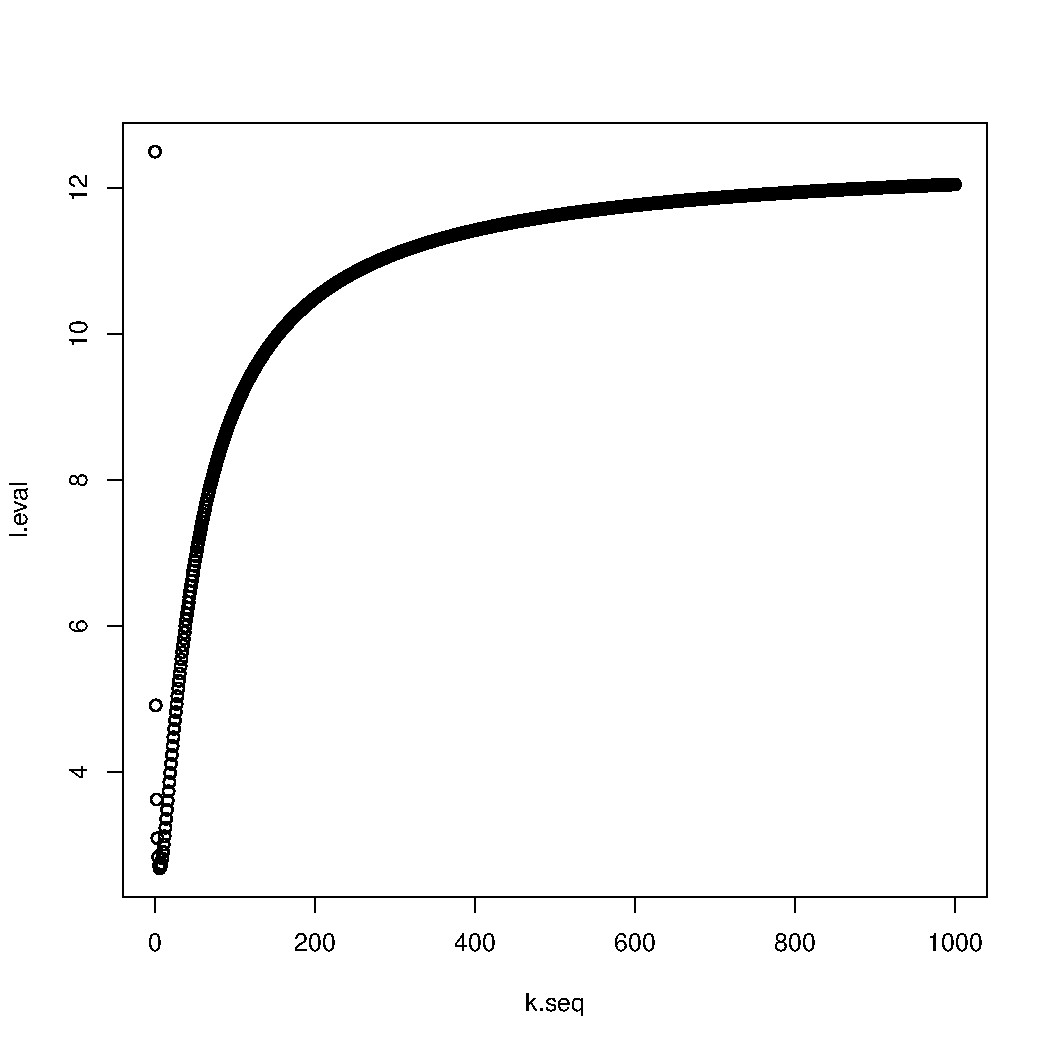
\includegraphics[width=\maxwidth]{figure/unnamed-chunk-11-1} 
\begin{kframe}\begin{alltt}
\hlstd{l.opt} \hlkwb{=} \hlkwd{optimize}\hlstd{(l.foo,} \hlkwd{c}\hlstd{(}\hlnum{0}\hlstd{,} \hlnum{100}\hlstd{), sig.sq, lambda, e.beta); l.opt}
\end{alltt}
\begin{verbatim}
## $minimum
## [1] 6.179617
## 
## $objective
## [1] 2.679957
\end{verbatim}
\end{kframe}
\end{knitrout}

\item

\begin{knitrout}
\definecolor{shadecolor}{rgb}{0.969, 0.969, 0.969}\color{fgcolor}\begin{kframe}
\begin{alltt}
  \hlstd{d_0} \hlkwb{=} \hlkwd{d.foo}\hlstd{(}\hlnum{0}\hlstd{, sig.sq, lambda, e.beta); d_0}
\end{alltt}
\begin{verbatim}
## [1] 15.36967
\end{verbatim}
\begin{alltt}
  \hlstd{d.opt}
\end{alltt}
\begin{verbatim}
## $minimum
## [1] 11.94841
## 
## $objective
## [1] 0.346172
\end{verbatim}
\begin{alltt}
  \hlstd{l_0} \hlkwb{=} \hlkwd{l.foo}\hlstd{(}\hlnum{0}\hlstd{, sig.sq, lambda, e.beta); l_0}
\end{alltt}
\begin{verbatim}
## [1] 12.5
\end{verbatim}
\begin{alltt}
  \hlstd{l.opt}
\end{alltt}
\begin{verbatim}
## $minimum
## [1] 6.179617
## 
## $objective
## [1] 2.679957
\end{verbatim}
\end{kframe}
\end{knitrout}

\qquad For D(k), D(k.opt)$<$D(0), it's possible to improve over the ordinary least squares method using ridge regression.
For L(k), L(k.opt)$<$L(0), which also means it's possible to improve over the ordinary least squares method using ridge regression.



\end{enumerate}

\end{document}
